\chapter{Obecný modul periferie}
\label{sec:modul-periferie}
    Díky zvolené koncepci systému je možné za periferii považovat jakékoliv zařízení schopné obousměrně komunikovat po navržené sběrnici. Není vyloučeno, aby byla každá periferie navržena zcela odlišně na základě svých vlastních požadavků na výkon, počet pinů nebo dostupná rozhraní daného MCU. Hlavní výhodou této koncepce je to, že periferie mohou být vyvíjeny postupně a přidávány do již funkčního a odladěného systému bez nutnosti modifikovat stávájící hardware. V~případě chyby v~návrhu periferie je také oprava méně náročná, než by tomu bylo v~případě zabudování veškeré funkcionality přímo do řídící jednotky. 

    Nicméně pokud by byl pro každou periferii zvolen zcela jiný mikrokontroler a vytvořen vlastní návrh DPS, vývoj více periferií by byl zbytečně drahý a časově náročný. Proto byl zvolen koncept \uv{obecného modulu periferie}, tedy jedné DPS s~konkrétním mikrokontrolerem zajišťující připojení ke komunikačního rozhraní, napájení periferie a rozhraní pro programování. Kromě toho budou na DPS dvě dutinkové lišty, do kterých bude možné vsadit druhou DPS (popř. během vývoje pouze prototypovací desku) ve funkci dceřinné desky (ang. daughterboard). Vložená deska pak bude obsahovat obvody nutné přímo pro danou konkrétní periferii.
    
    \section{Mikrokontrolér}

        Kritéria pro výběr mikrokontroleru byla následující:
        \begin{itemize}
            \item Musí nutně splňovat:
            \begin{itemize}
                \item CAN periferie -- pro komunikaci po sběrnici 
                \item PWM výstup -- řízení LED, popř. jiné
                \item ADC -- pro práci s analogovými sensory
                \item Nízká cena 
            \end{itemize}
            \item Je výhodou:
            \begin{itemize}
                \item Dobrá dokumentace, komunita uživatelů
                \item Zkušenost autora s~danou platformou
                \item Další periferie (\acs{i2c}, SPI, ...)
            \end{itemize}
        \end{itemize}

        Na základě těchto kritérií byl vybrán mikrokontroler \textbf{PIC18F26Q83} od firmy Microchip, ten splňuje všechna kritéria a disponuje také množstvím dalších periferií, které by mohly být v~budoucnu užitečné~\cite{PIC18F26Q83}.

    \section{Návrh zapojení a tvorba DPS}
        Celé schéma pro obecný modul periferie se nachází v příloze~\ref{priloha:schema-modul-periferii}. Návrh zapojení lze rozdělit na tři části. V prvním kroku je zapojen mikrokontroler tak, aby byly opět splněny všechny požadavky výrobce. Mikrokontrolery řady PIC se vyznačují značnou jednoduchostí použití a ke správnému chodu jim stačí jen minimum dalších součástek. V případě PIC18F26Q83 postačí připojit blokovací kondenzátor (C6) na napájení (pin VCC) a přivést kladné napětí na resetovací pin (MCLR). MCU je dále doplněn resetovacím tlačítkem pro pohodlnější práci při vývoji a testování firmwaru a regulátorem napětí (U1) s výstupem \qty{3.3}{V}. 

        Ve druhém kroku je přidána dvojice D'sub konektorů a CAN řadič ATA6561 obdobně jako u řídící jednotky popsané v sekci \ref{sec:ridici-jednotka-schema-a-dps}. Na závěr jsou všechny dosud nevyužité piny vyvedeny na konektor (dutinkovou lištu), aby byly jednoduše dostupné pro připojenou dceřinnou desku. Pro napájení výkonově náročnejších periferií (např. ovladač LED osvětlení) jsou zvlášť vyvedeny ještě dvě trojice pinů připojené na \qty{24}{V} a zem (GND).

        \subsubsection{Tvorba DPS}
        Hlavním cílem bylo vytvořit DPS co nejmenší. Jedná se o samostatné moduly, kterých bude v systému zapojeno několik a pro manipulaci a rozmístění modulů okolo akvária je menší rozměr výhodou. Hlavní limitací v této snaze není počet součástek, ale spíše rozměry mechanických prvků, zejména konektorů D'sub. Na obr.~\ref{fig:modul-periferie-dps} je vidět výsledný návrh DPS s osazenými součástkami a dosaženými rozměry. Je zřejmé že jiným rozložením dutinkových lišt by se návrh dal ještě drobně zmenšit, ale je potřeba ponechat jistou flexilitu pro tvorbu dceřinných desek.

        \begin{figure}[!ht]
            \centering
            \begin{tikzpicture}
                % Include the image
                \node[anchor=south west,inner sep=0] (image) at (0,0) {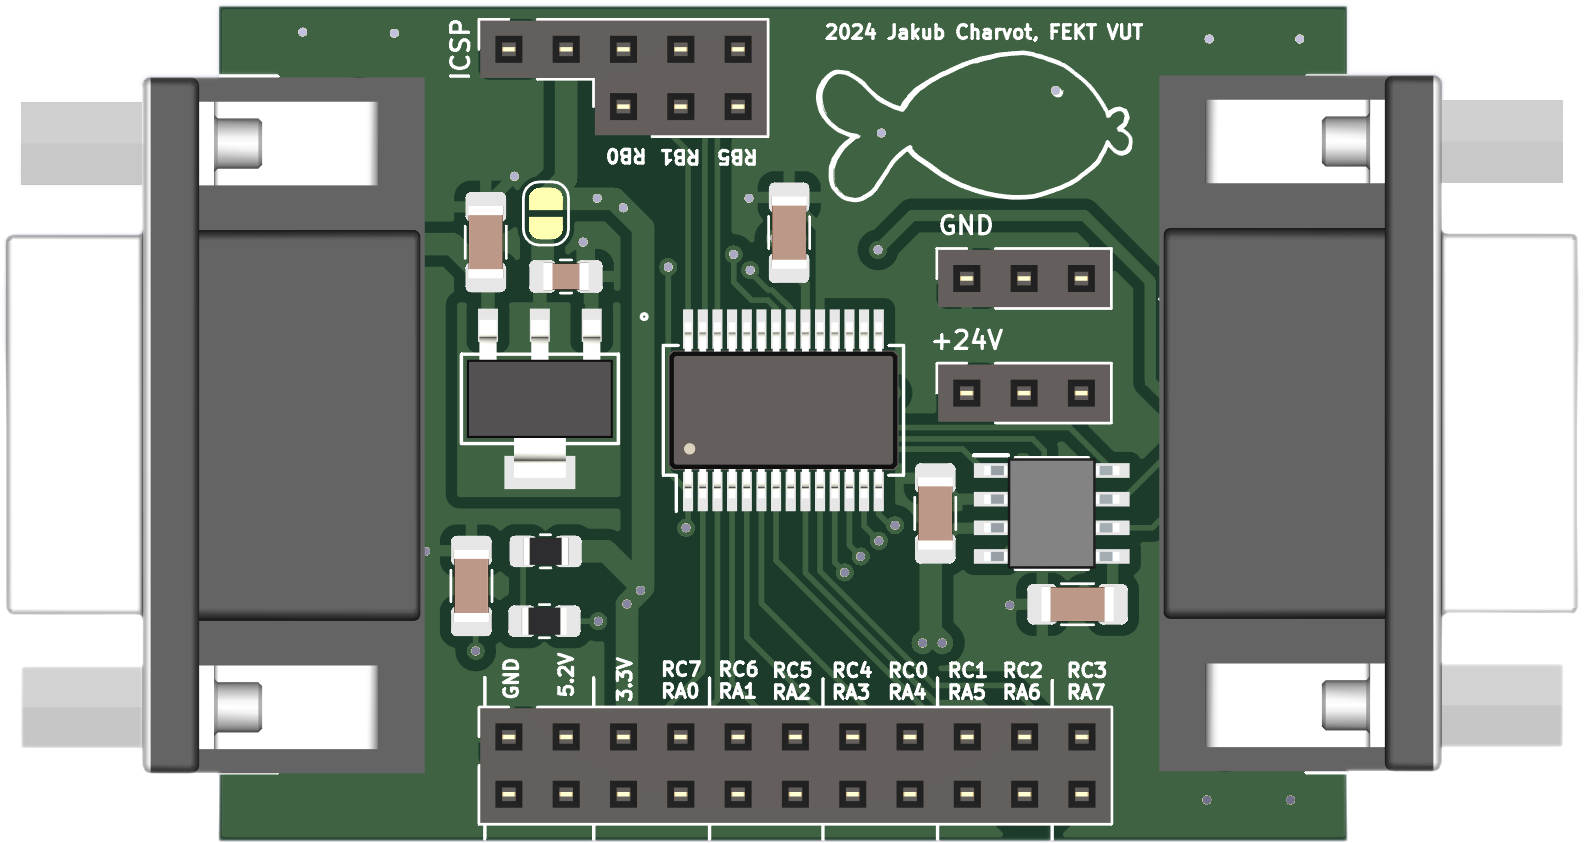
\includegraphics[width=0.8\textwidth]{obrazky/dps/peripherial-module-3d-top.png}};
                
                \draw[dashed] (10.1,0.04) -- (12.5,0.04);
                \draw[<->,thick] (12.5,0.04) -- (12.5,6.34);
                \draw[dashed] (12.5,6.34) -- (10.1,6.34);
                \node[anchor=west] at (12.5,3.15)  {\qty{36}{mm}};

                \draw[dashed] (1.12,0.64) -- (1.12,-0.5);
                \draw[<->,thick] (1.12,-0.6) -- (10.9,-0.6);
                \draw[dashed] (10.9,-0.6) -- (10.9,0.64);
                \node[anchor=south] at (6,-0.6)  {\qty{57}{mm}};
            \end{tikzpicture}
            \caption{Vizualizace DPS obecného modulu periferie.}
            \label{fig:modul-periferie-dps}
        \end{figure}

        Co se týče rozložení vrstev, byla opět použita čtyřvrstvá deska se strejnou strukturou jako je na obr.~\ref{fig:ridici-jednotka-stackup-dps} pro DPS řídící jednotky. Celý návrh DPS se nachází v příloze TODO.



